\chapter{Malware and malware samples}

First of all, before addressing the question of what a ``malware sample'' is,
let us analyze what a ``malware'' is.

The National Institute of Standards and Technologies (NIST) throws the
following definition of malware: ``Software or firmware intended to perform an
unauthorized process that will have adverse impact on the confidentiality,
integrity, or availability of an information system. A virus, worm, Trojan
horse, or other code-based entity that infects a host. Spyware and some forms
of adware are also examples of malicious
code.''\cite{Nist2013}

And RFC4949\cite{Rfc4949} defines
``malicious logic'' as ``Hardware, firmware, or software that is intentionally
included or inserted in a system for a harmful purpose.''

A lot of definitions of ``malware'' do
exist\cite{NistGlossary2020} but in this work we propose to use this one to remark some key points of
malware nature:
\begin{tcolorbox}
  Any element, hardware, software and/or firmware, determined malicious in
  some context and in a state of its life cycle.
\end{tcolorbox}

Notice that proposed malware definition has a strong subjective component
because it is not possible to say if something is malicious in a fully
objective way\cite{LayeredDetectionMethod}.  Therefore, an element is not inherently malicious. Instead, an
element is determined malicious in a state of its life cycle and taking into
account the context.

To clarify this idea with an example: the TCP/IP swiss army knife
\texttt{netcat} does not seem to be designed specifically with malicious
purposes so, if context is ignored, it must be classified as goodware. But,
installed by an attacker and with the purpose of giving access to a remote
computer, this tool must clearly be classified as malware. It is in these
cases considered inconclusive (and in some others cases not relevant here) in
which industry uses intermediate terms such as ``riskware'', ``hacktool'',
``grayware'' or ``potentially unwanted program''.

\begin{figure}
  \centering
  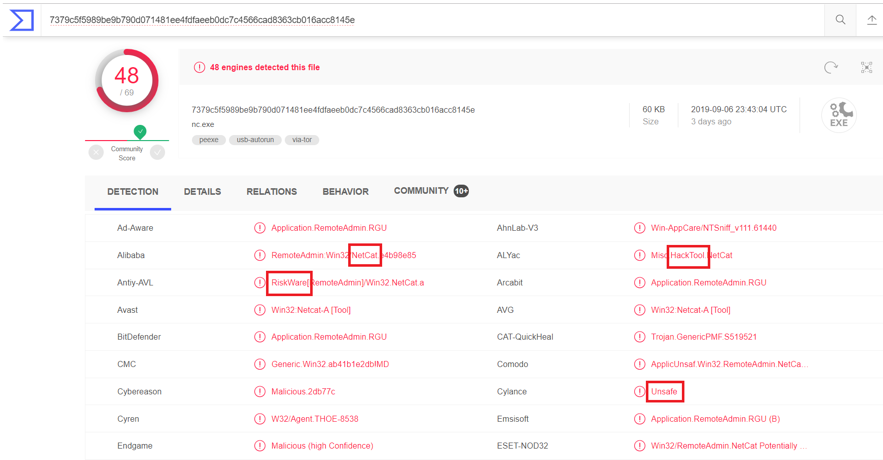
\includegraphics[width=0.99\textwidth]{./figures/Image1.png}
  \caption{\label{fig:1} An illustration of a VirusTotal analysis of Netcat.}
\end{figure}

Malware context is absolutely fundamental during analysis\cite{ContextBasedMalware}\cite{LearningFromContext} so, it must to be
included in the collected samples. The concept of malware sample is broad,
since its nature consists of a composition of miscellaneous elements\cite{ResidentViruses}\cite{FilelessAttacks}\cite{AdvacedVolatileThreat}. We must,
therefore, include different kind of elements (memory dumps, files, pictures
and circuit specifications in case of hardware malware, network traffic
captures, environment variables, etc.) and to enrich these elements with
metadata to indicate the analyst what exactly is any kind of element
appended as metadata as necessary.

In contradiction with any definition of ``malware'', currently a ``malware
sample'' is any kind of file that, potentially, could be malware. In other
words, and to keep it simple, malware samples are not always malware. Let us
clarify this issue next.

\section{The state of the art in malware samples}
\label{sec:soa}

It is known that intelligence tools simply store files, without any rigor of
selection beyond self-tagging by the user who, while it is true, accepts the
EULA (End User License Agreement), probably desiring strongly that potential
sensitive data are properly encrypted.

In the same way, antimalware solutions also take malware samples from the
system of its clients and, with high probability, all the undetected and
unknown elements, because new detections cannot come from other place than the
knowledge acquired from the unknown and undetected samples. Therefore, those
files are paradoxically also called malware samples. This is not a new
thing. For instance, Kaspersky Antivirus has starred the news not long ago on
this issue\cite{RussianStoleNsaSpySecrets}\cite{KasperskyToolForSpying}.  This
highlights that pointing to Kaspersky Antivirus as espionage tool by EE.UU and
EU is not other thing than to accidentally discover the general lack of
current malware sample treatment in general, not by a specific company or
product. In other words, a treatment which does not take into account, among
other issues not at all negligible, data confidentiality and user privacy.

This incident meant great losses, leading Kaspersky to create a ``Transparency
Center''\cite{KasperskyTransparencyCenter} and Eugene Kaspersky, CEO of Kaspersky Lab, to publish many releases like
this: ``We’re even willing to meet with any of them and give them our source
code to thoroughly review it, as we’ve got nothing to
hide''\cite{EugeneKasperskyBlog2017}. Certainly, Kaspersky antivirus is not a spy tool by itself (as happens with
any software piece, it depends on the context, it depends on who uses it), you
can check the entire source code line by line and you will not notice
specifically designed code for espionage, but you will notice the real issue:
samples treatment! And no direct actions were taken in this sense by antivirus
industry because, if it is not well done, it can reduce the protection rate
that, unfortunately, is the only thing the customer demands.

We reproduce as en example two EULA blocks chosen at random because to quote
all will be too much extensive and repetitive. These are quite similar for all
antivirus companies and products.

\begin{tcolorbox}
  \small
  12.1 The Software or Support may employ applications and tools to collect
  Personal Data, sensitive data or other information about Company and End
  Users (including End Users’ name, address, e-mail address and payment
  details), their computers, files stored on their computers, or their
  computers’ interactions with other computers (including information
  regarding network, licenses used, hardware type, model, hard disk size, CPU
  type, disk type, RAM size, 32 or 64 bit architecture, operating system
  types, versions, locale, BIOS version, BIOS model, total scanners deployed,
  database size, system telemetry, device ID, IP address, location, content,
  McAfee products installed, McAfee components, processes and services
  information, frequency and details of update of McAfee components,
  information about third party products installed, extracts of logs created
  by McAfee, usage patterns of McAfee products and specific features, etc.)
  (collectively,
  Data).\footnote{\href{https://www.mcafee.com/enterprise/en-us/assets/legal/end-user-license-agreements-en-us.pdf}{\texttt{https://www.mcafee.com/enterprise/en-us/assets/legal/end-user-license-agreements-en-us.pdf}}}
  
  \tcblower
  SECTION B. CONDITIONS REGARDING DATA PROCESSING

  Provision of information (if applicable) In order to enhance the protection
  of information and improve the quality of the Software and services, You
  agree to automatically provide Kaspersky Lab with the following information
  of a statistical and administrative nature: information about installed
  programs, license data, information on detected threats and infections,
  checksums of processed objects, technical information about the Computer and
  devices connected to it, information about online activity of the device as
  well as You agree that such information can be provided to third-party
  service providers. More information is available at help.kaspersky.com.  In
  order to identify new information security threats and their sources,
  enhance the operational protection of Users of the Software, and improve the
  quality of the product, You agree to automatically provide Kaspersky Lab
  with information specified in the Terms of Use of Kaspersky Security
  Network.  Also, You can activate and deactivate the Kaspersky Security
  Network service at any time in the Software settings window.  You further
  acknowledge and agree that any information gathered by Rightholder can be
  used to track and publish reports on security risk trends at the
  Rightholder’s sole and exclusive discretion.  If you do not wish to provide
  information to the Kaspersky Security Network service, You should not
  activate the Kaspersky Security Network service. If service is already
  activated, you should immediately de-activate the Kaspersky Security Network
  service.

  Kaspersky Lab protects the information received in accordance with
  applicable governing law and Kaspersky Lab's rules. Data is transmitted over
  a secure channel.\footnote{\href{https://products.s.kaspersky-labs.com/homeuser/kav2020/20.0.14.1085abc/english-INT-0.2007.0/3231373433327c44454c7c4e554c4c/eula_en.txt}{\texttt{https://products.s.kaspersky-labs.com/homeuser/kav2020/20.0.14.1085abc/english-INT-0.2007.0/3231373433327c44454c7c4e554c4c/eula_en.txt}}}
\end{tcolorbox}
As you can read from its own words: sensitive data is collected. You can check
not only literature but also the code to verify this.

\section{Antivirus telemetry}

\subsection{Analysis}
Our starting hypothesis is that any antimalware solution is an espionage tool
in potential, and that not only files are sent to the server but also
intelligence information that can be used to spy the users.

Let us do some reverse engineering on an antivirus product in order to know
what kind of information is sent to the company. Let us do this with
\texttt{Malwarebytes} because telemetry DLL is very easy to identify, this is
actually the main reason to chose this antivirus product for investigating the
issue.

\begin{figure}[t]
  \centering
  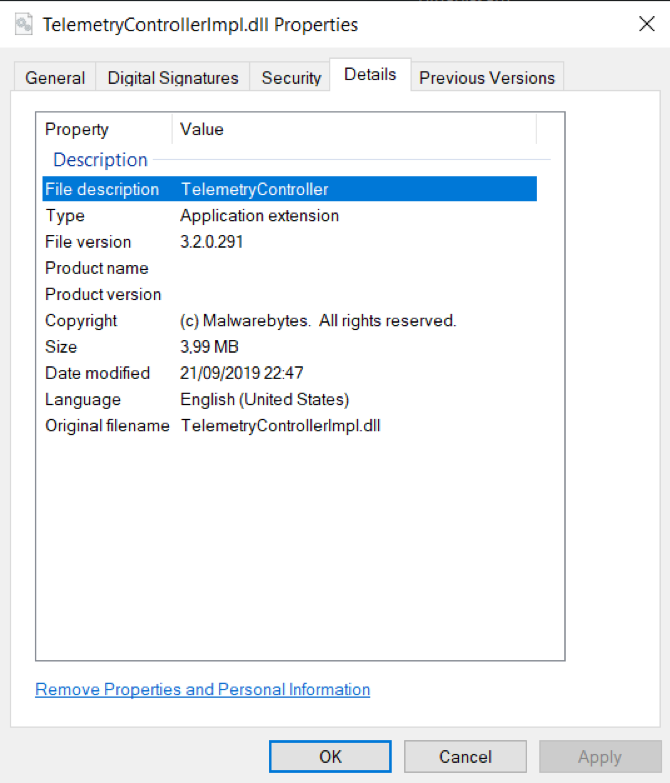
\includegraphics[width=0.85\textwidth]{./figures/ControllerImpl}
  \caption{\label{fig:ControllerImpl} Reverse engineering in
    \texttt{Malwarbytes}.}
\end{figure}
The file responsible of \texttt{Malwarebytes} antivirus telemetry is the
\begin{tcolorbox}
  \texttt{TelemetryControllerImpl.dll}
\end{tcolorbox}
shown in Figure~\ref{fig:ControllerImpl}. If we take a look at the exported
functions, we can see what kind of information is collected
(Figure~\ref{fig:ExportedFunction}).

\begin{figure}
  \centering
  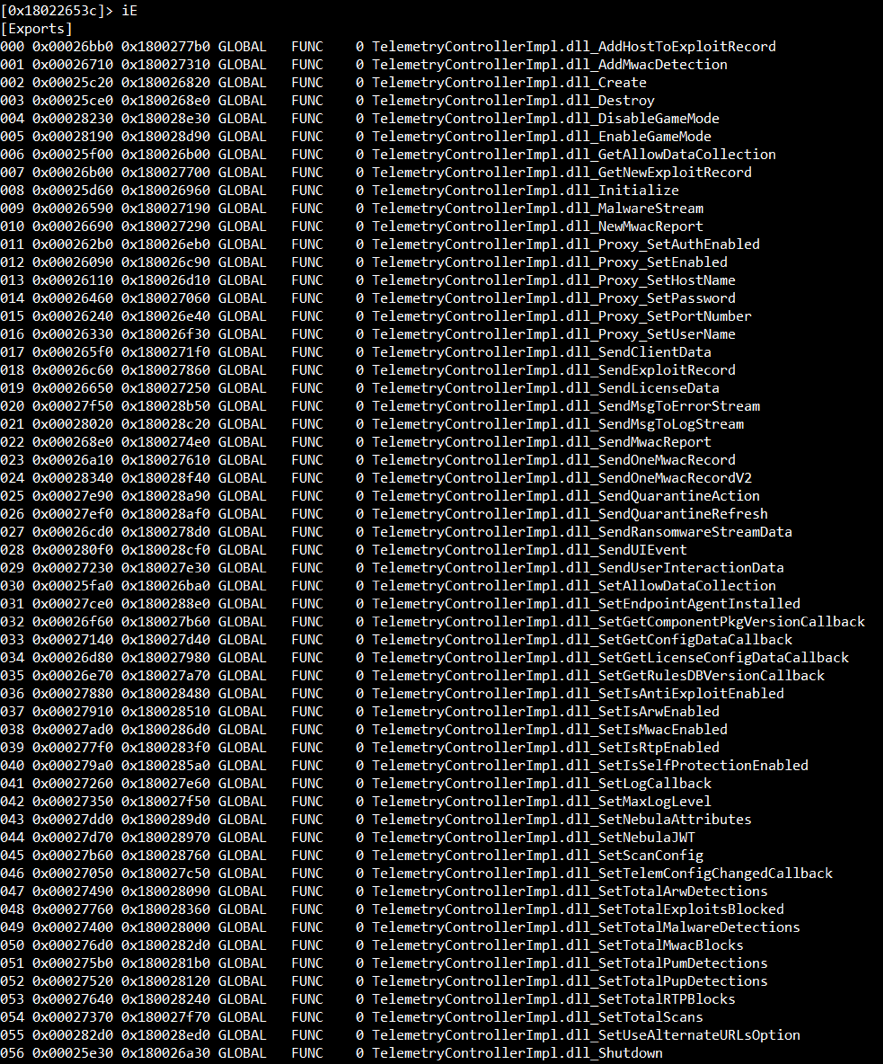
\includegraphics[width=0.85\textwidth]{./figures/ExportedFunction}
  \caption{\label{fig:ExportedFunction} Exported functions.}
\end{figure}

This list of exported function names seems to be self-explanatory, and it
reveals without obfuscation what kind of information is sent. It can be
summarized as follows.
\begin{itemize}
\item Malware information (ransomware is treated in its own specific way).
\item Exploits information.
\item Client data.
\item License data.
\item Error information.
\item Quarantine information.
\item Statistics.
\end{itemize}
We can also contrast the summary developed above with every of the third endpoint path
names of the \texttt{Malwarebytes} telemetry exposed API, shown in Figure~\ref{fig:api}.
\begin{figure}[t]
  \centering
  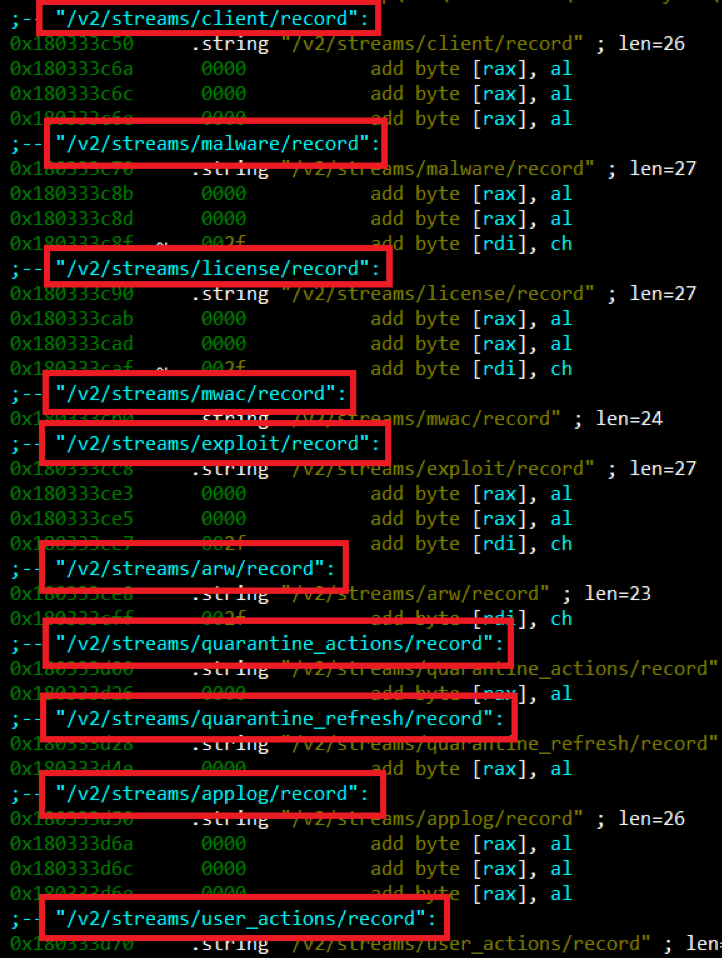
\includegraphics[width=0.80\textwidth]{./figures/Malwarebytes}
  \caption{\label{fig:api} \texttt{Malwarebytes} telemetry API.}
\end{figure}
The endpoint path is the following:
\href{https://telemetry.malwarebytes.com/api}{\texttt{https://telemetry.malwarebytes.com/api}}
and, as an off-topic observation, the development endpoint is also publicly
exposed:
\href{https://telemetry.dev.malwarebytes.com/api}{\texttt{https://telemetry.dev.malwarebytes.com/api}}. 

We can also examine some function of those (\texttt{SendMwacReport}, for
instance, has an interesting name) in order to understand how are samples
treated in terms of confidentiality. This function sends a JSON file
\texttt{mwcstream.json} using Microsoft Winsocks library.
\begin{figure}[h]
  \centering
  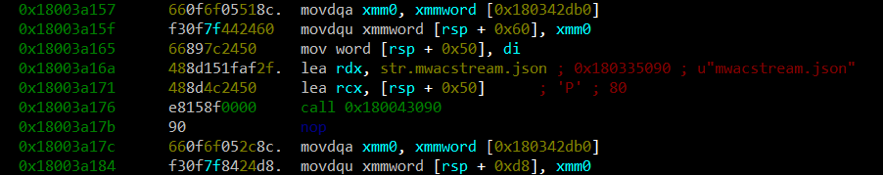
\includegraphics[width=0.99\textwidth]{./figures/mwcstream}
\end{figure}

The function responsible of the ``send'' action is
\begin{tcolorbox}
\texttt{TelemetryControllerImpl::SendMwacReport}
\end{tcolorbox}
as shown in the following disassembly listing:
 \begin{figure}[h]
  \centering
  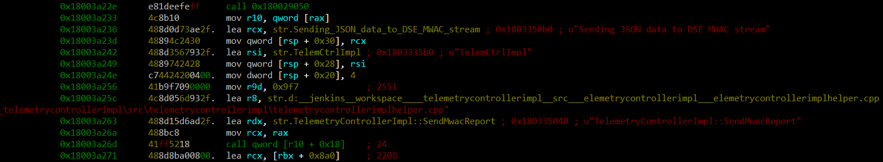
\includegraphics[width=0.99\textwidth]{./figures/SendMwacReport}
\end{figure}

We can take another function from the list and we can see that all information
is sent in the same way. It uses also a JSON file (in this case it is named
\texttt{malwarestream.json}):
\begin{figure}[h]
  \centering
  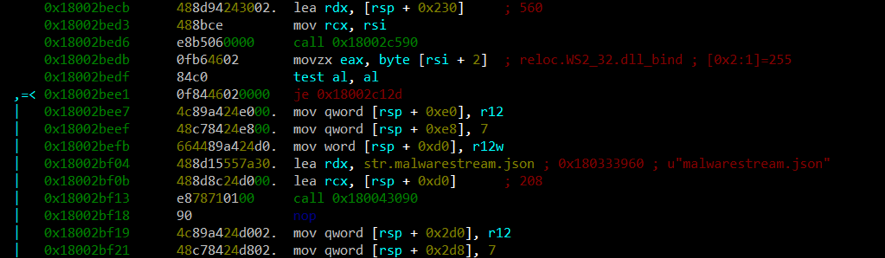
\includegraphics[width=0.99\textwidth]{./figures/malwarestream}
\end{figure}

And finally the appropriate report sending function for this kind of JSON
structure, \texttt{TelementryControllerImpl::ReportMalwareStream} in this
case:
 \begin{figure}[h]
  \centering
  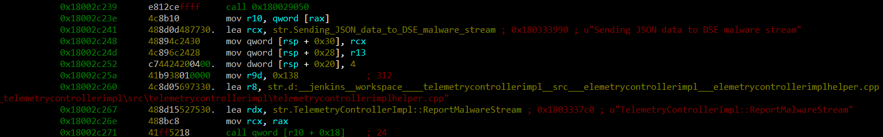
\includegraphics[width=0.99\textwidth]{./figures/ReportMalwareStream}
\end{figure}

Our next step is debug \texttt{Malwarebytes} in order to see how this JSON
looks like. For instance, we can break in some point inside the function
\texttt{SendOneMwacRecordV2} after analyzing (on demand) a file infector, and
see the information.
\begin{figure}[h]
  \centering
  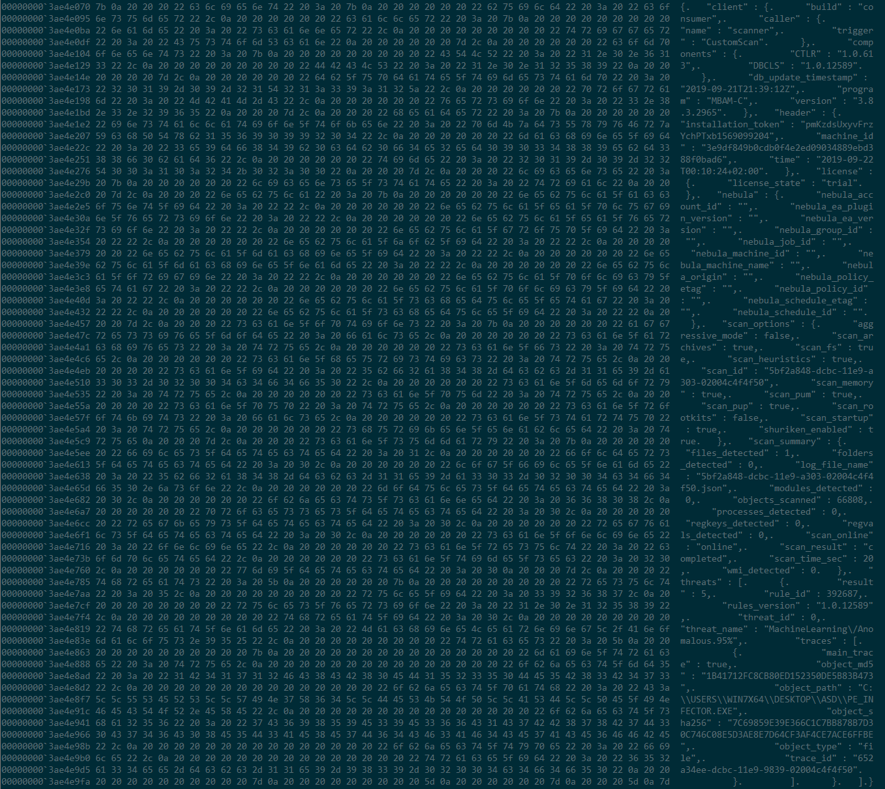
\includegraphics[width=0.99\textwidth]{./figures/Debug1}
\end{figure}
As you can see, apart of malware sample itself, other information is collected
separately, unencrypted and stored in a non-standard format. We remark that
the computer where these tests have been performed can be easily tracked by
checking the unique identifier \texttt{machine\_id}. Into the binary
\texttt{.rdata} section a series of WMI queries do exist for machine
identification purposes.
\begin{figure}
  \centering
  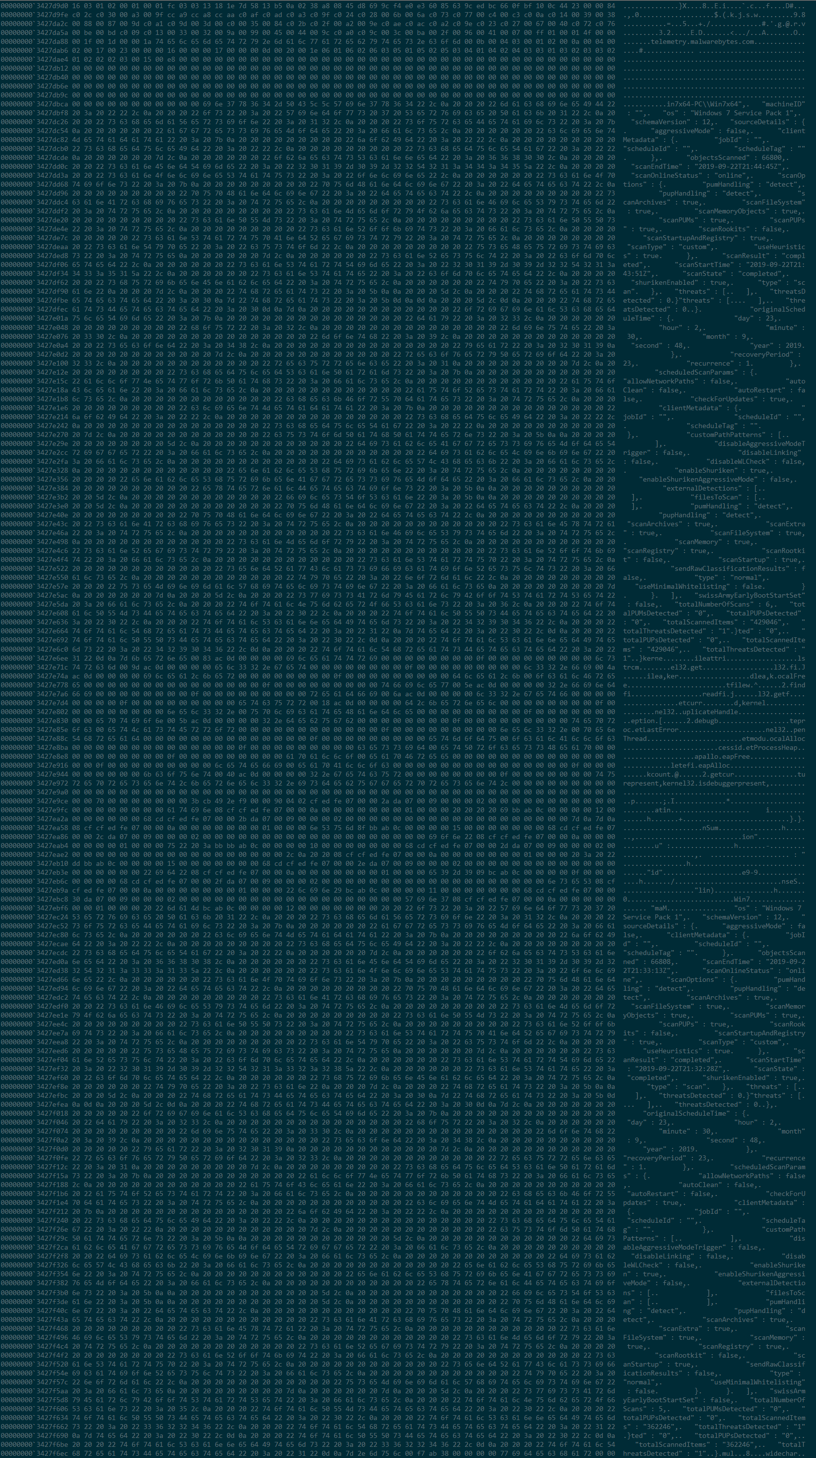
\includegraphics[width=0.85\textwidth]{./figures/Debug2}
  \caption{\label{fig:malwarebytes-debug} Debugging \texttt{Malwarebytes}.}
\end{figure}

\begin{tcolorbox}
  \small
\begin{verbatim}
SELECT Index, MACAddress, Name FROM Win32_NetworkAdapter 
       where AdapterTypeId=0
SELECT UUID FROM Win32_ComputerSystemProduct
SELECT processorID FROM win32_processor
SELECT SerialNumber FROM Win32_BIOS
SELECT Signature FROM Win32_DiskDrive WHERE Index=%u
SELECT serialNumber FROM Win32_PhysicalMemory
SELECT SerialNumber FROM Win32_DiskDrive WHERE Index=%u
\end{verbatim}
\end{tcolorbox}

Since Microsoft Winsock functions are used for network communications, we can
also break in \texttt{Send} and \texttt{SendTo} functions and show de buffer
content before telemetry data are sent
(Figure~\ref{fig:malwarebytes-debug}). It is as easy as stated because the
\texttt{Malwarebytes} self-defense is not enabled just after installing the
product, a really hilarious security bug which can be used to attack the
debugger without bypassing any kind of protection.


The file responsible of Malwarebytes antivirus cloud functionality is the
\texttt{CloudControllerImpl.dll}.
\begin{figure}[h]
  \centering
  \includegraphics[width=0.7\textwidth]{./figures/CloudcontrollerImpl}
\end{figure}


Let us follow the same analysis steps with this file. Now, export listing looks as
follows:
\begin{figure}[h]
  \centering
  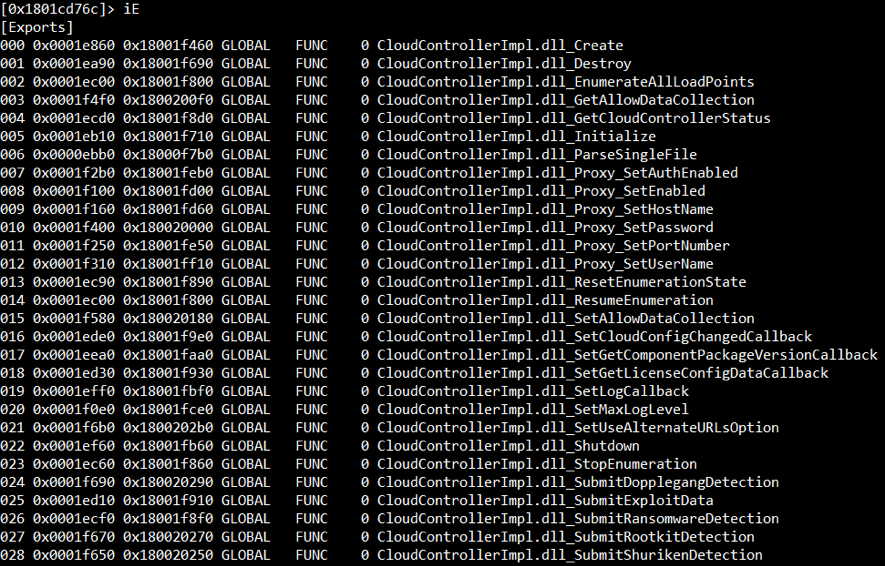
\includegraphics[width=0.7\textwidth]{./figures/ExportListing}
\end{figure}

There are five functions at the very end of the screenshot named starting by
the prefix \texttt{Submit}. Those functions are responsible of submitting
files and memory chunks to the \texttt{Malwarebytes} cloud storage, but those
functions are only called when upgrading to the premium version of the
product\cite{MalwarebytesUserGuide}.  
\begin{figure}[h]
  \centering
  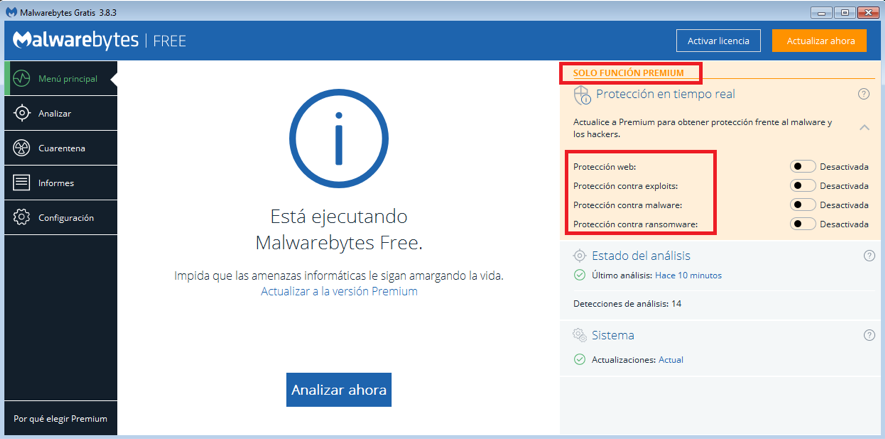
\includegraphics[width=0.99\textwidth]{./figures/MalwareBytesFree}
\end{figure}

The reader should know what ``exploit'', ``ransomware'', and ``rootkit'' mean,
but there are two function names which maybe seem a little stranger:

\noindent\texttt{SubmitDopplegangDetection} and \texttt{SubmitShurikenDetection}
because they are \texttt{Malwarebytes} specific terms. The first one,
\texttt{SubmitDopplegangDetection}, as you can see in the following picture,
is used to send ``scam'' detections:
\begin{figure}[h]
  \centering
  \includegraphics[width=0.75\textwidth]{./figures/Scamdetection}
\end{figure}

But \texttt{SubmitShurikenDetection} is much more interesting for us, because
it is used to send heuristically detected samples, meaning, by definition,
that false positives will absolutely happens (goodware files are potentially
sent to the cloud storage).
\begin{figure}[h]
  \centering
  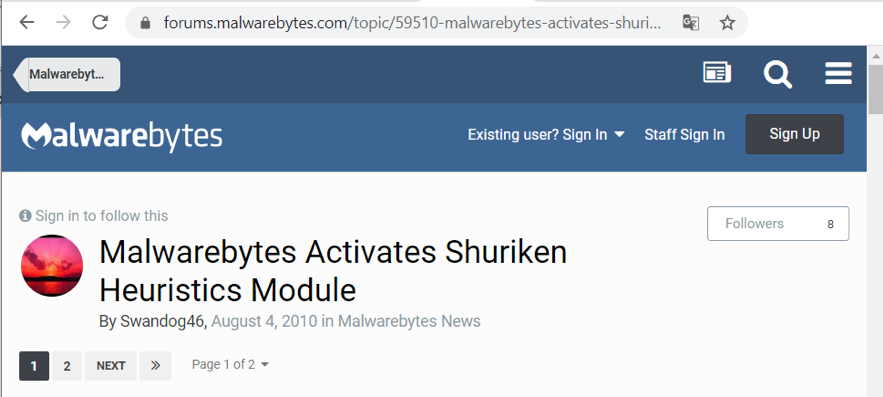
\includegraphics[width=0.75\textwidth]{./figures/SubmitShurikenDetection}
\end{figure}

All of this information is submited to the following endpoints:
\begin{tcolorbox}
  \small
  \href{https://bactem-staging.mwbsys.com/files}{\texttt{https://bactem-staging.mwbsys.com/files}} \\
  \href{https://staging-blitz.mb-cosmos.com/}{\texttt{https://bactem-staging.mwbsys.com/files}} \\
  \href{https://blitz.mb-cosmos.com/}{\texttt{https://blitz.mb-cosmos.com/}} \\
  \href{https://static-blitz.mb-cosmos.com/}{\texttt{https://static-blitz.mb-cosmos.com/}}
  \\ 
  \href{https://blitz.mb-cosmos.com/}{\texttt{https://blitz.mb-cosmos.com/}} \\
  \href{https://static-blitz.mb-cosmos.com/}{\texttt{https://static-blitz.mb-cosmos.com/}}
\end{tcolorbox}
If the reader is interested about where those files are stored, we can also
answer this question. These files are stored in the server referenced by the
following IP address: \texttt{3.229.68.76} and it corresponds to Amazon Data
Services NoVa:
%\begin{figure}[h]
%  \centering
%  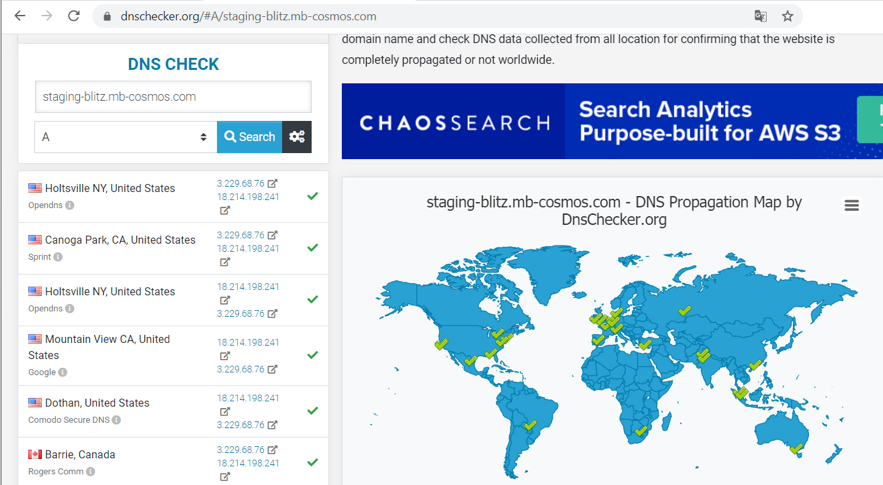
\includegraphics[width=0.75\textwidth]{./figures/DNScheck}
%\end{figure}

\begin{figure}[h]
  \centering
  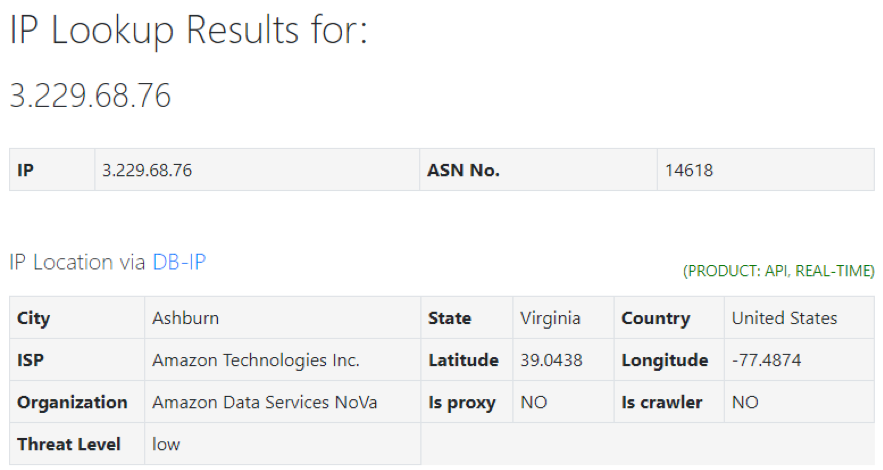
\includegraphics[width=0.75\textwidth]{./figures/Lookup}
\end{figure}

This is an important point because the code is developed using Amazon S3
API\cite{AmazonS3RestApi}.
The following is a little fragment of the \texttt{Shuriken} sending function:
\begin{figure}[h]
  \centering
  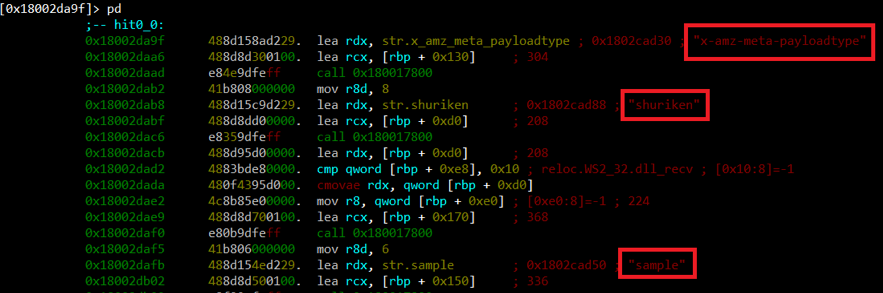
\includegraphics[width=0.99\textwidth]{./figures/Shuriken}
\end{figure}

As you can see, \texttt{x-amz-meta-payloadtype} is the ``payloadtype'' custom
metadata parameter prefixed as specified by Amazon S3 API, and the rest means
that a \texttt{Shuriken} sample submission is happening.
\begin{figure}[h]
  \centering
  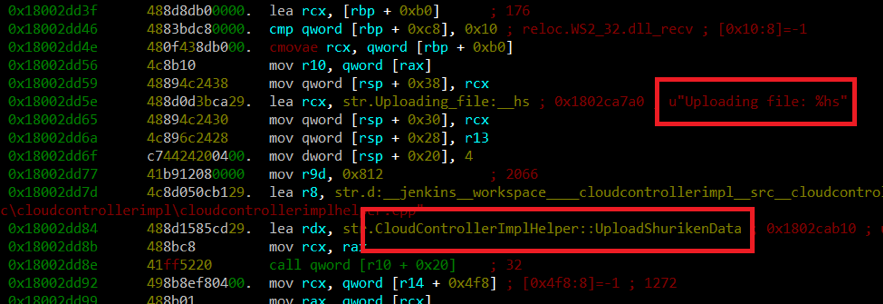
\includegraphics[width=0.99\textwidth]{./figures/Shuriken2}
\end{figure}

Thus, we have identified the mechanism used to send samples and telemetry data
to the \texttt{Malwarebytes} cloud server. Another interesting thing is to
know how file and memory samples are chosen by this product in order to keep
them in the server. Following the natural analysis flow, some interesting
functions are located into \texttt{MBAMService.exe} which finally relies on
\texttt{CloudControllerImpl.dll} where all the hard job takes place.
\begin{figure}[h]
  \centering
  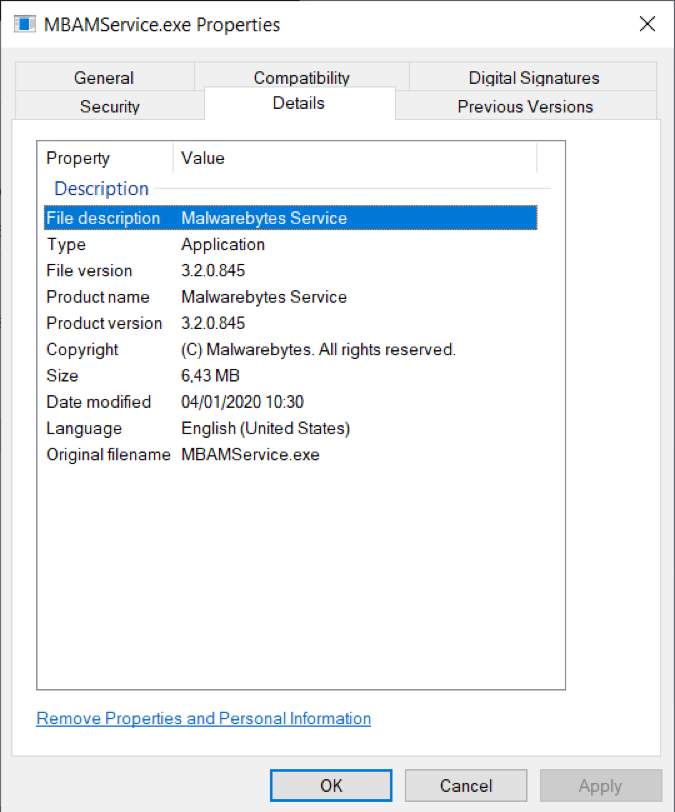
\includegraphics[width=0.75\textwidth]{./figures/MBAMService}
\end{figure}

There are a lot of callbacks into this binary image. Two of them make
reference to cloud submission and telemetry submission, specifically:
\begin{figure}[h]
  \centering
  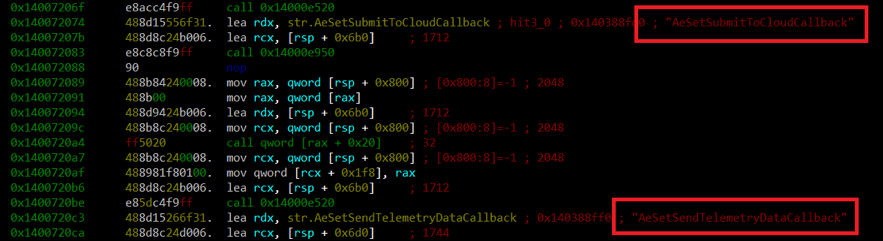
\includegraphics[width=0.99\textwidth]{./figures/Callbacks}
\end{figure}

If reader is really interested about how \texttt{Malwarebytes} heuristically
chooses files to be sent to the cloud storage, remember that when using
heuristics, by definition, no categorical conclusions are possible so false
positives will happen. Therefore, confidential files in addition to potential
malware embedding confidential data could be sent to the server. It is
recommended to the restless reader to disassemble
\texttt{CloudControllerImpl.dll} by his/her own to perform a further analysis.

At this point, it is necessary to install \texttt{Malwarebytes} Premium in
order to investigate the file submission features. We obtained a trial\cite{MalwarebytesPremium} license
for a limited period.  In this Premium Trial version, real-time features are
available. We noticed that this \texttt{Malwarebytes} version has more sample
submission routines, and identified the following sample submission exports in
the \texttt{CloudControllerImpl.dll} library file:
\begin{enumerate}
\item \texttt{SubmitDDSSample}
\item \texttt{SubmitDopplegangDetection}
\item \texttt{SubmitExploitData}
\item \texttt{SubmitMWACDetection}
\item \texttt{SubmitQuarantineRestoreItem}
\item \texttt{SubmitRansomwareDetection}
\item \texttt{SubmitRootkitDetection}
\item \texttt{SubmitShurikenDetection}
\end{enumerate}
The first thing we are interested in to investigate is how samples are
submitted. To this end, we executed a portable executable file infector and
broke into the \texttt{send} function of \texttt{WS2\_32.dll} to see how the
buffer content looks like.
\begin{figure}[h]
  \centering
  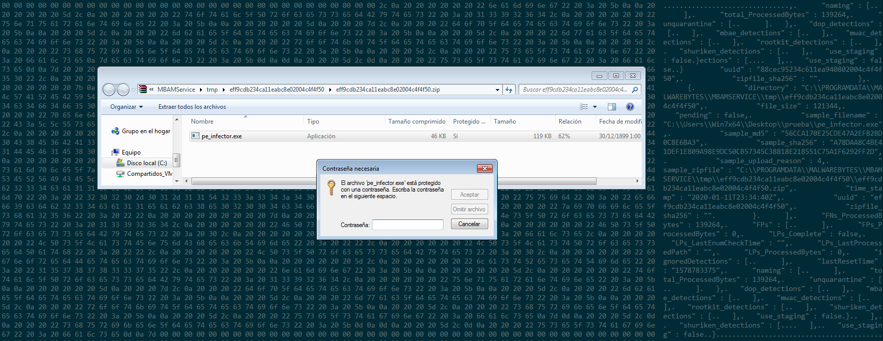
\includegraphics[width=0.99\textwidth]{./figures/Submission}
\end{figure}

As you can see in the JSON structure of the previous image, the sample file is stored into the following location:

\noindent{\small\verb|{C:\PROGRAMDATA\MALWAREBYTES\MBAMSERVICE\tmp\{hash_sha256}\{hash_sha256}.zip|}

\noindent This is a PKZIP file encrypted with the typical malware sample
password: ``infected''\cite{ZeltserShareMalware}.  And it will be sent to the Amazon server
\begin{tcolorbox}
  \texttt{btoc-samples-prod.s3.amazonaws.com}.
\end{tcolorbox}
The hypothesis that files are submitted is confirmed. The other thing we are
interested in to investigate is if \texttt{Malwarebytes} indiscriminately
submits all files or not.  Since a ``hello world'' program should never lead
to a false positive, if it is submitted, it can be assumed that submissions
are done indiscriminately.
\begin{figure}[h]
  \centering
  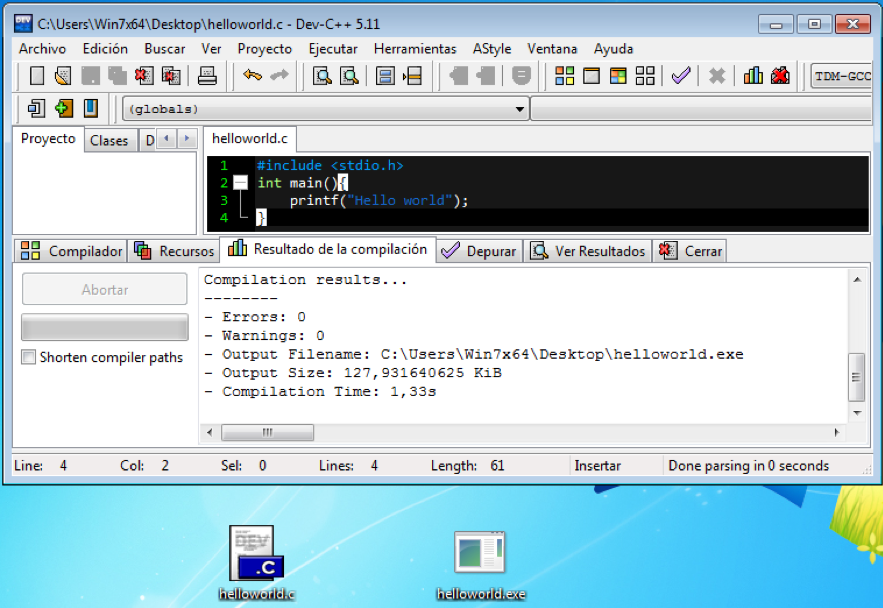
\includegraphics[width=0.99\textwidth]{./figures/HelloWorld}
\end{figure}

The experiment result indicated that, when \texttt{helloworld.exe} was
executed, some information was sent to \texttt{Malwarebytes} by using
\texttt{WS2\_32.dll} library \texttt{send} function with the call flow coming
from somewhere inside \texttt{RTPControllerImpl.dll}. This library contains
the following strings: \pagebreak
\begin{figure}[h]
  \centering
  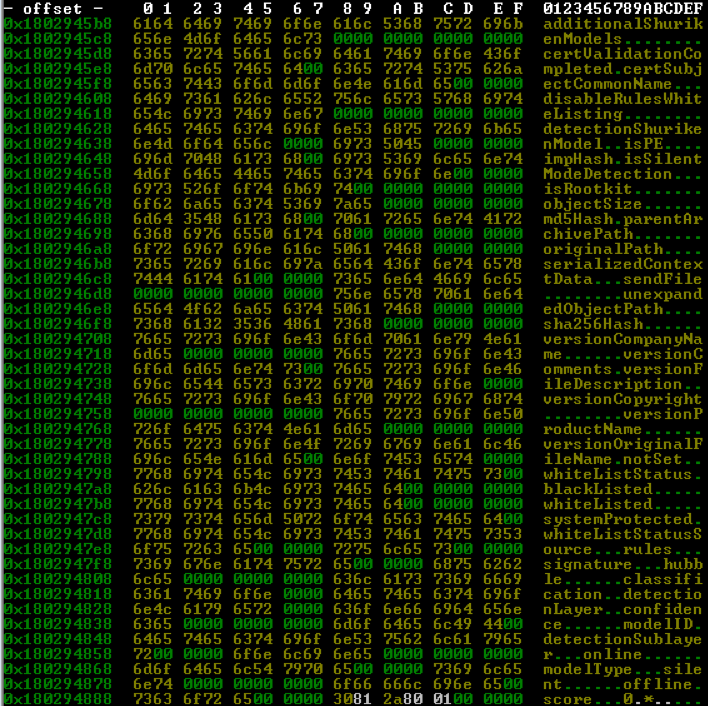
\includegraphics[width=0.85\textwidth]{./figures/Strings}
\end{figure}

\begin{figure}
  \centering
  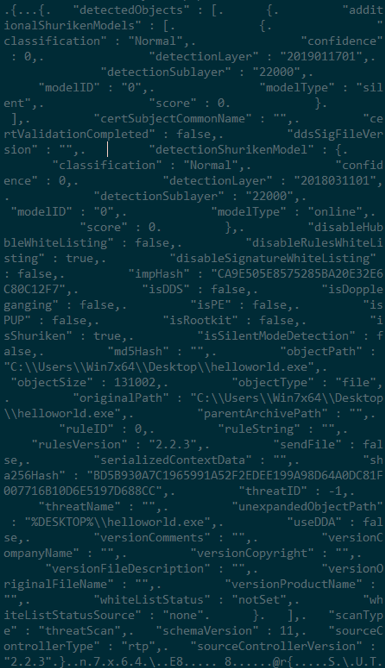
\includegraphics[width=0.6\textwidth]{./figures/ExperimentJSON}
  \caption{\label{fig:ExperimentJSON} Sample of the JSON experiment.}
\end{figure}
A function of \texttt{RTPControllerImpl} uses it to generate the
JSON. Experiment JSON looks as in Figure~\ref{fig:ExperimentJSON}.  So,
\texttt{Malwarebytes} Premium sends file samples only if it suspects a file
could be infected (a \texttt{sample\_upload\_reason} field do exist into the
JSON structure).  If the file is not a suspicious one, \texttt{Malwarebytes}
Premium sends information about the file (like the file path and something
like this) but not the file content itself. Anyway, subjectively, in our
opinion, executable files leak a lot of information about the user behavior.

\subsection{Conclusions}
The reverse engineering of the \texttt{Malwarebytes} antivirus products
reveals that these are not especially intrusive. They are classical
antiviruses with cloud features which send suspicious files and telemetry to
the cloud server just for purposes of comparison.

Our analysis indicates that some files (but, with congratulations to
\texttt{Malwarebytes}, not an indiscriminate massive volume of goodware ones)
are sent to the company's cloud server powered by Amazon.

Sample submission is done by using a PKZIP file protected with the typical
malware sample password: ``infected''\cite{ZeltserShareMalware}. And metadata information (telemetry) is
sent separately using a JSON format.  On the other hand, the most important
thing is that accessed goodware information is sent, the user is unambiguously
identified and some information is collected apart of the sample file itself.
If such collected information were accessed, for instance, by a third party
like an unethical employee or a government intelligence agency (which maybe
collaborates with the antivirus company and could take advantage of this fact)
they could track a specific user (or users, in general) and combine this
information with other databases (including another antivirus products)\cite{KasperskyBoundariesOfTrust}.
\texttt{Malwarebytes} could substantially improve its system by removing both,
the compressed samples system and the telemetry data. Instead, it could
progressively add sample and telemetry support to the UMSE dynamic linking
library and call to it before submitting samples.

\section{Cyber threat hunting telemetry and samples submission}

\subsection{Analysis}

Cyber threat hunting is defined as follows: ``the process of proactively and
iteratively searching through networks to detect and isolate advanced threats
that evade existing security solutions''.

In practice, cyber threat hunting means to capture as many events as possible,
correlate them and send reports of them all the time. All the magic can be
summarized in one sentence: everything can be detected if everything is
real-time reviewed.
\begin{figure}
  \centering
  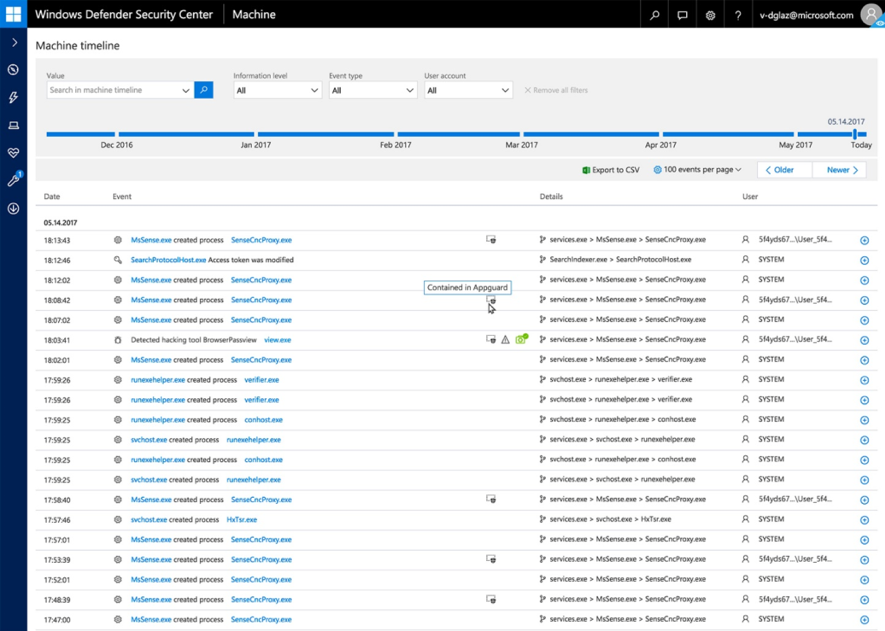
\includegraphics[width=0.75\textwidth]{./figures/WindowsDefender}
  \caption{\label{fig:WindowsDefender} A screenshot of WindowsDefender.}
\end{figure}

For instance, Windows Defender Advanced Threat Protection captures the
following information\cite{MicrosoftDefenderAtp2020}, as shown in Figure~\ref{fig:WindowsDefender}:\footnote{\href{https://docs.microsoft.com/en-us/windows/security/threat-protection/microsoft-defender-atp/advanced-hunting-schema-reference}{https://docs.microsoft.com/en-us/windows/security/threat-protection/microsoft-defender-atp/advanced-hunting-schema-reference}}
\begin{enumerate}
\item Alerts on Microsoft Defender Security Center.
\item Machine information, including OS information.
\item Network properties of machines, including adapters, IP and MAC
  addresses, as well as connected networks and domains.
\item Process creation and related events.
\item Network connection and related
  events.
\item File creation, modification, and other file system events.
\item Creation and modification of registry entries.
\item Sign-ins and other authentication events.
\item DLL loading events.
\item Multiple event types, including events triggered by security controls
  such as Windows Defender Antivirus and exploit protection.
\end{enumerate}
The idea is the same for all products. Event correlation is an important
feature. Check Figure~\ref{fig:CarbonBlack}, as an example, taken out of from the
\texttt{Carbon Black}\cite{CarbonBlack2017} tool.
\begin{figure}
  \centering
  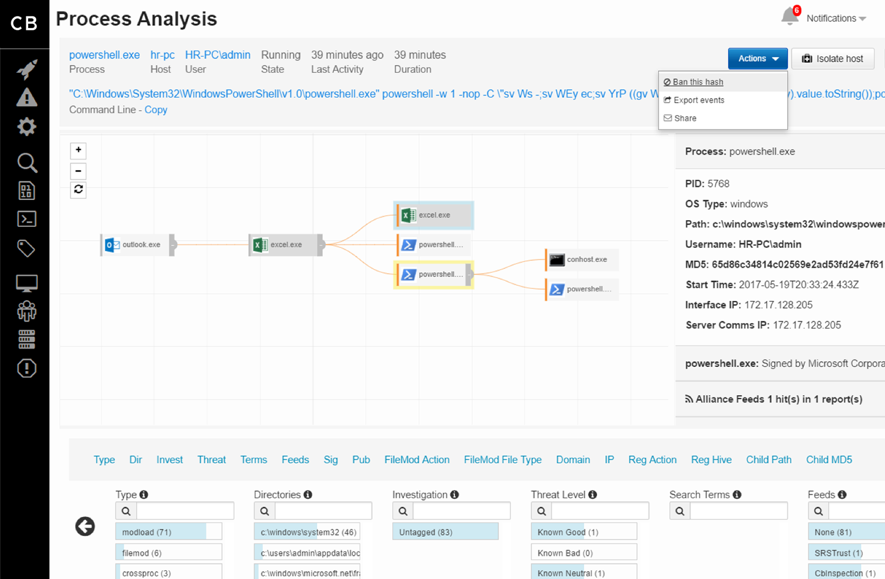
\includegraphics[width=0.99\textwidth]{./figures/CarbonBlack}
  \caption{\label{fig:CarbonBlack} Source: \href{https://www.carbonblack.com/wp-content/uploads/2017/04/BanHash-B.png}{\texttt{https://www.carbonblack.com/wp-content/uploads/2017/04/BanHash-B.png}}}
\end{figure}

\subsection{Conclusion}

It is hard to imagine a more aggressive kind of security tools in terms of
user data confidentiality. More detections but unjustifiably much less
confidentiality.  You can check pictures publicly available in Google of this
kind of tools, most of them will be carefully chosen by the manufacturer
(meaning that the aggressive behavior will be as hidden as possible) but if
one watches the dashboard containing event logs of those tools, one will soon
realize how powerful they are in terms of surveillance. You will see a steady
stream of events unrelated to malware.  Threat hunting tools could also
substantially improve their system by adding events, files, processes,
registry keys and support for system elements into the UMSE dynamic linking
library, and by calling to its API before submitting collected data.

\section{Operating system telemetry and samples submission}

\subsection{Analysis}

Next, we want to explore what happens if there are no additional antivirus
software installed in the computer. Must the user be worried about security
products that maybe come built-in the operating system? And, if these are
disabled, must the user be worried about other security products installed in
the local area network (LAN) because of firewall telemetry and sample
submission capabilities?

The Microsoft Windows telemetry DLL file is located in
\begin{tcolorbox}
  \verb|C:\Windows\System32\generaltel.dll|.
\end{tcolorbox}
\begin{figure}[h]
  \centering
  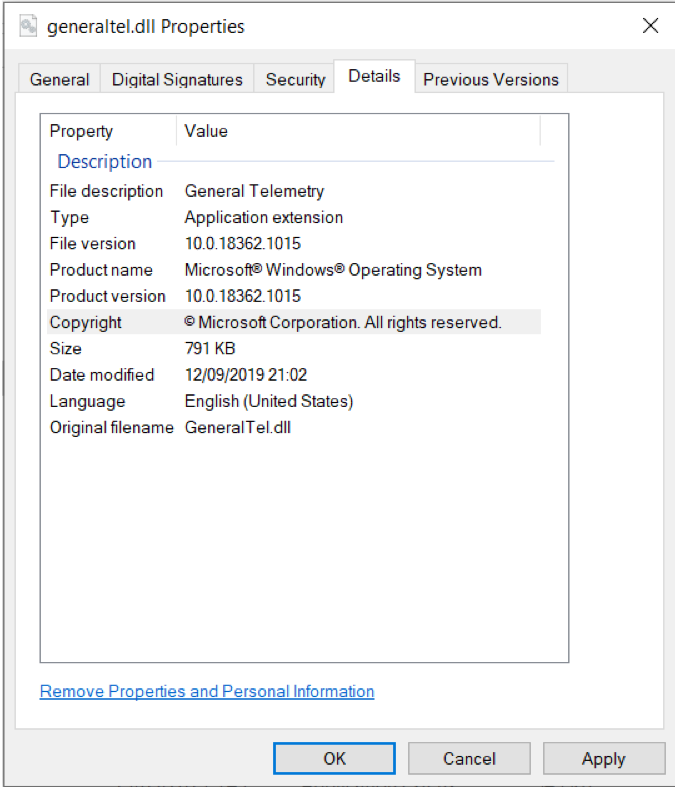
\includegraphics[width=0.6\textwidth]{./figures/WindowsTelemetry}
\end{figure}

And you will readily notice that miscellaneous antivirus, antispyware and
firewall information is sent to Microsoft, where \texttt{Firewall information}
means network information. It is possible to disable all the telemetry but
maybe your LAN neighbor does not do that.
\begin{figure}[h]
  \centering
  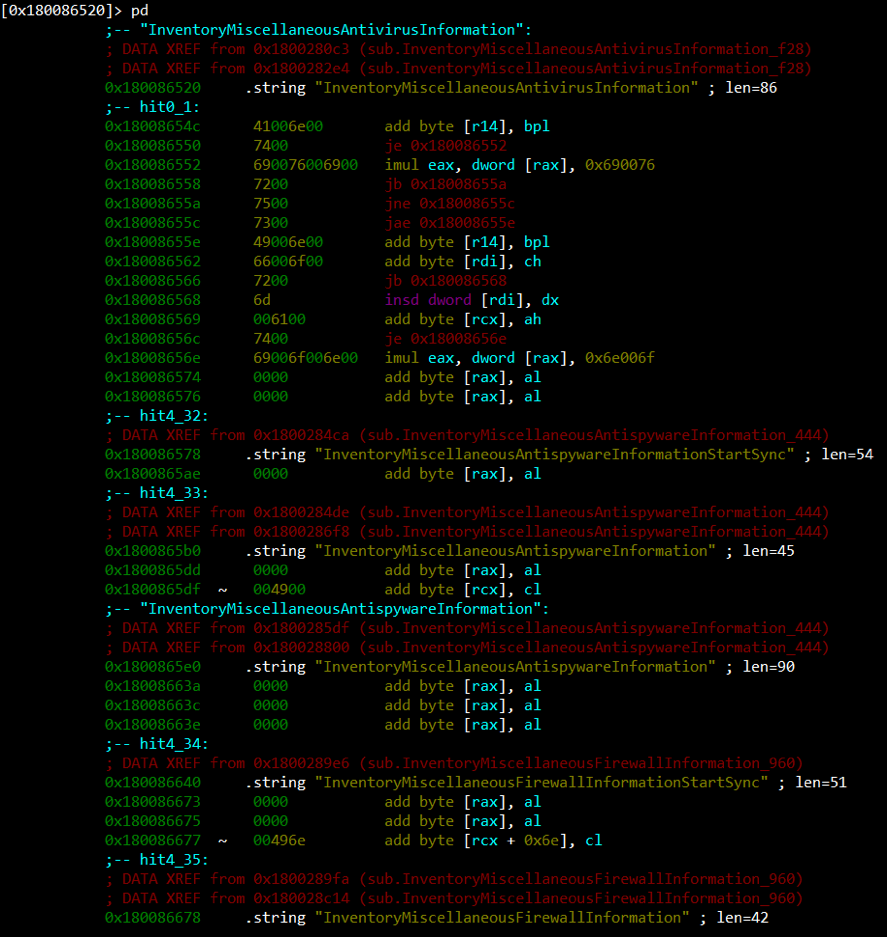
\includegraphics[width=0.99\textwidth]{./figures/MiscellaneousAntivirus}
\end{figure}

The cloud submission features of sample files also do exist and they are
customizable by the user. It is possible to check easily (without reverse
engineering nothing) what kind of information is sent to Microsoft because,
due to open criticism, they released a tool named \texttt{Diagnostic Data
  Viewer}. You can use it immediately for those purposes (Figure~\ref{fig:libUmse}).
\begin{figure}[h]
  \centering
  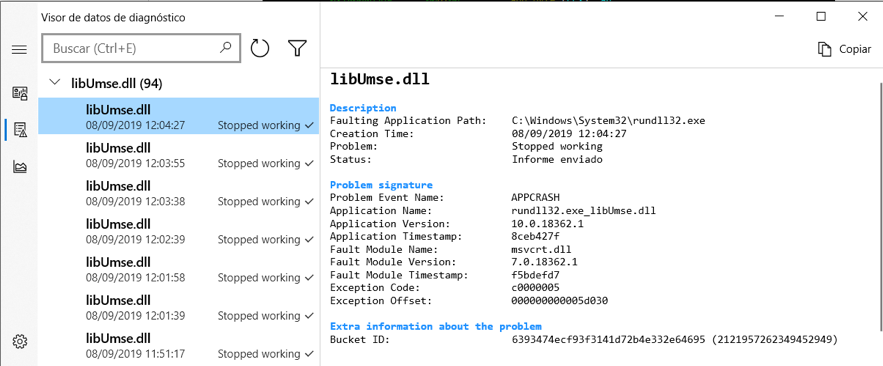
\includegraphics[width=0.75\textwidth]{./figures/libUmse}
  \caption{\label{fig:libUmse} libUmse.dll}
\end{figure}

In the lab computer used for this work, minimum telemetry is allowed which
means that antimalware telemetry is disabled but nevertheless crashes allow
Microsoft to follow the development of this thesis in real-time. Someone might
think that this assessment is unrelated to malware but information about
crashes is also used for this\cite{MicrosoftRdpCrashes2019} (see Figure~\ref{fig:rdp})
purpose.\footnote{\href{https://www.microsoft.com/security/blog/2019/11/07/the-new-cve-2019-0708-rdp-exploit-attacks-explained/}{https://www.microsoft.com/security/blog/2019/11/07/the-new-cve-2019-0708-rdp-exploit-attacks-explained/}}
\begin{figure}[h]
  \centering
  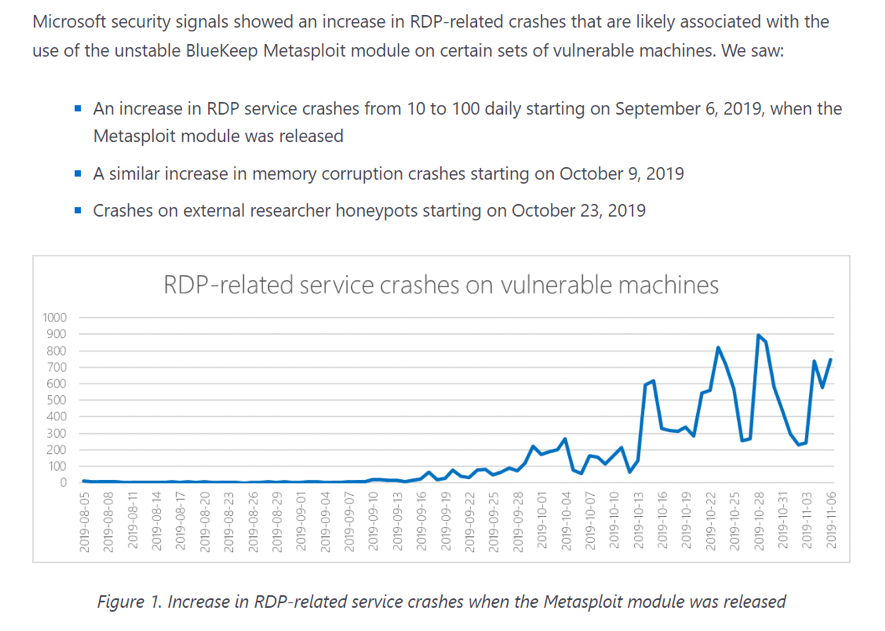
\includegraphics[width=0.8\textwidth]{./figures/RDP}
  \caption{\label{fig:rdp}}
\end{figure}

\subsection{Conclusion}

Some operating systems contain built-in antimalware/firewall/threat hunting
solutions. It is difficult for the common user to disable telemetry
capabilities. A minimum telemetry is required by the operating system (and
seems to be used also for malware purposes). Antivirus, antispyware and
firewall information is sent meaning that also LAN network information can be
revealed.  Operating system antimalware/firewall/threat hunting solutions
could also substantially improve its system by adding events, files,
processes, registry keys and system elements support into the UMSE dynamic
linking library and calling to it before submitting collected data.

\section{Intelligence products}

\subsection{Analysis}

Malware intelligence tools store goodware in, maybe, greater volume than
malware.  \texttt{VirusTotal} is a service which allows you to check if a file
is malware or not by querying a lot of antivirus engines.  If you search,
e.g.,''tutorial pdf'' in Google, (a reasonable random goodware file), the
first result, in this case, is a Python Tutorial PDF. Finally, if you check if
this file does exist in \texttt{VirusTotal}, you can see that it does (really,
a lot of files are in \texttt{VirusTotal}, this can be checked
straightforwardly). So, any person with a \texttt{VirusTotal} paid API account
can download this file, make advanced searches in binaries (including Yara
search) and easily locate files\cite{VirusTotalFileSearch2020}. It is true that people who submits files
accepts the EULA but, as you can see, if you have the paid \texttt{VirusTotal}
API you can download books, software, movies \dots. Those old determined
goodware files, some even signed, will be never removed from storage.

\subsection{Conclusion}

Malware intelligence tools store goodware in, maybe, greater volume than
malware\cite{IntrusionDetectionNetworks}. Those are not malware samples, those are simple, ordinary files.
Intelligence products could also substantially improve its system by adding
encryption support for uncommon and copyrighted likely goodware files (because
those files are not interesting for malware analysis in any way, not even to
be compared with infected files) into the UMSE dynamic linking library. In
this way, only files detected by at least one antimalware engine or a reliable
human should be decrypted and opened to the world.

%%% Local Variables:
%%% mode: latex
%%% TeX-master: "thesis"
%%% End:
